\documentclass[letterpaper, 10pt, draftclsnofoot, compsoc, onecolumn]{IEEEtran}


\usepackage{graphicx}
%\usepackage{amssymb}
%\usepackage{amsmath}
%\usepackage{amsthm}

\usepackage{alltt}
\usepackage{float}
\usepackage{url}

\usepackage{balance}
\usepackage[TABBOTCAP, tight]{subfigure}
\usepackage{enumitem}
\usepackage{pstricks, pst-node}

\usepackage{hyperref}
\usepackage{geometry}

\usepackage{comment}
\setcounter{tocdepth}{4}
\setcounter{secnumdepth}{4}

\usepackage{listings}
\usepackage{color}
\usepackage[doublespacing]{setspace}
\usepackage{supertabular}
\usepackage{fancyhdr}

%\setlength{\parindent}{4em}
%\linespread{1.1}

\pagestyle{empty}
\renewcommand{\headrulewidth}{0pt}
\lhead{Many Voices Publishing Platform}

\lfoot{SDD}
\cfoot{Page}
\rfoot{\thepage}

\def\name{Steven Powers, Josh Matteson, Evan Tschuy}

%pull in the necessary preamble matter for pygments output
%\usepackage{fancyvrb}
\usepackage{color}
\usepackage[latin1]{inputenc}


\makeatletter
\def\PY@reset{\let\PY@it=\relax \let\PY@bf=\relax%
    \let\PY@ul=\relax \let\PY@tc=\relax%
    \let\PY@bc=\relax \let\PY@ff=\relax}
\def\PY@tok#1{\csname PY@tok@#1\endcsname}
\def\PY@toks#1+{\ifx\relax#1\empty\else%
    \PY@tok{#1}\expandafter\PY@toks\fi}
\def\PY@do#1{\PY@bc{\PY@tc{\PY@ul{%
    \PY@it{\PY@bf{\PY@ff{#1}}}}}}}
\def\PY#1#2{\PY@reset\PY@toks#1+\relax+\PY@do{#2}}

\expandafter\def\csname PY@tok@gd\endcsname{\def\PY@tc##1{\textcolor[rgb]{0.63,0.00,0.00}{##1}}}
\expandafter\def\csname PY@tok@gu\endcsname{\let\PY@bf=\textbf\def\PY@tc##1{\textcolor[rgb]{0.50,0.00,0.50}{##1}}}
\expandafter\def\csname PY@tok@gt\endcsname{\def\PY@tc##1{\textcolor[rgb]{0.00,0.25,0.82}{##1}}}
\expandafter\def\csname PY@tok@gs\endcsname{\let\PY@bf=\textbf}
\expandafter\def\csname PY@tok@gr\endcsname{\def\PY@tc##1{\textcolor[rgb]{1.00,0.00,0.00}{##1}}}
\expandafter\def\csname PY@tok@cm\endcsname{\let\PY@it=\textit\def\PY@tc##1{\textcolor[rgb]{0.25,0.50,0.50}{##1}}}
\expandafter\def\csname PY@tok@vg\endcsname{\def\PY@tc##1{\textcolor[rgb]{0.10,0.09,0.49}{##1}}}
\expandafter\def\csname PY@tok@m\endcsname{\def\PY@tc##1{\textcolor[rgb]{0.40,0.40,0.40}{##1}}}
\expandafter\def\csname PY@tok@mh\endcsname{\def\PY@tc##1{\textcolor[rgb]{0.40,0.40,0.40}{##1}}}
\expandafter\def\csname PY@tok@go\endcsname{\def\PY@tc##1{\textcolor[rgb]{0.50,0.50,0.50}{##1}}}
\expandafter\def\csname PY@tok@ge\endcsname{\let\PY@it=\textit}
\expandafter\def\csname PY@tok@vc\endcsname{\def\PY@tc##1{\textcolor[rgb]{0.10,0.09,0.49}{##1}}}
\expandafter\def\csname PY@tok@il\endcsname{\def\PY@tc##1{\textcolor[rgb]{0.40,0.40,0.40}{##1}}}
\expandafter\def\csname PY@tok@cs\endcsname{\let\PY@it=\textit\def\PY@tc##1{\textcolor[rgb]{0.25,0.50,0.50}{##1}}}
\expandafter\def\csname PY@tok@cp\endcsname{\def\PY@tc##1{\textcolor[rgb]{0.74,0.48,0.00}{##1}}}
\expandafter\def\csname PY@tok@gi\endcsname{\def\PY@tc##1{\textcolor[rgb]{0.00,0.63,0.00}{##1}}}
\expandafter\def\csname PY@tok@gh\endcsname{\let\PY@bf=\textbf\def\PY@tc##1{\textcolor[rgb]{0.00,0.00,0.50}{##1}}}
\expandafter\def\csname PY@tok@ni\endcsname{\let\PY@bf=\textbf\def\PY@tc##1{\textcolor[rgb]{0.60,0.60,0.60}{##1}}}
\expandafter\def\csname PY@tok@nl\endcsname{\def\PY@tc##1{\textcolor[rgb]{0.63,0.63,0.00}{##1}}}
\expandafter\def\csname PY@tok@nn\endcsname{\let\PY@bf=\textbf\def\PY@tc##1{\textcolor[rgb]{0.00,0.00,1.00}{##1}}}
\expandafter\def\csname PY@tok@no\endcsname{\def\PY@tc##1{\textcolor[rgb]{0.53,0.00,0.00}{##1}}}
\expandafter\def\csname PY@tok@na\endcsname{\def\PY@tc##1{\textcolor[rgb]{0.49,0.56,0.16}{##1}}}
\expandafter\def\csname PY@tok@nb\endcsname{\def\PY@tc##1{\textcolor[rgb]{0.00,0.50,0.00}{##1}}}
\expandafter\def\csname PY@tok@nc\endcsname{\let\PY@bf=\textbf\def\PY@tc##1{\textcolor[rgb]{0.00,0.00,1.00}{##1}}}
\expandafter\def\csname PY@tok@nd\endcsname{\def\PY@tc##1{\textcolor[rgb]{0.67,0.13,1.00}{##1}}}
\expandafter\def\csname PY@tok@ne\endcsname{\let\PY@bf=\textbf\def\PY@tc##1{\textcolor[rgb]{0.82,0.25,0.23}{##1}}}
\expandafter\def\csname PY@tok@nf\endcsname{\def\PY@tc##1{\textcolor[rgb]{0.00,0.00,1.00}{##1}}}
\expandafter\def\csname PY@tok@si\endcsname{\let\PY@bf=\textbf\def\PY@tc##1{\textcolor[rgb]{0.73,0.40,0.53}{##1}}}
\expandafter\def\csname PY@tok@s2\endcsname{\def\PY@tc##1{\textcolor[rgb]{0.73,0.13,0.13}{##1}}}
\expandafter\def\csname PY@tok@vi\endcsname{\def\PY@tc##1{\textcolor[rgb]{0.10,0.09,0.49}{##1}}}
\expandafter\def\csname PY@tok@nt\endcsname{\let\PY@bf=\textbf\def\PY@tc##1{\textcolor[rgb]{0.00,0.50,0.00}{##1}}}
\expandafter\def\csname PY@tok@nv\endcsname{\def\PY@tc##1{\textcolor[rgb]{0.10,0.09,0.49}{##1}}}
\expandafter\def\csname PY@tok@s1\endcsname{\def\PY@tc##1{\textcolor[rgb]{0.73,0.13,0.13}{##1}}}
\expandafter\def\csname PY@tok@sh\endcsname{\def\PY@tc##1{\textcolor[rgb]{0.73,0.13,0.13}{##1}}}
\expandafter\def\csname PY@tok@sc\endcsname{\def\PY@tc##1{\textcolor[rgb]{0.73,0.13,0.13}{##1}}}
\expandafter\def\csname PY@tok@sx\endcsname{\def\PY@tc##1{\textcolor[rgb]{0.00,0.50,0.00}{##1}}}
\expandafter\def\csname PY@tok@bp\endcsname{\def\PY@tc##1{\textcolor[rgb]{0.00,0.50,0.00}{##1}}}
\expandafter\def\csname PY@tok@c1\endcsname{\let\PY@it=\textit\def\PY@tc##1{\textcolor[rgb]{0.25,0.50,0.50}{##1}}}
\expandafter\def\csname PY@tok@kc\endcsname{\let\PY@bf=\textbf\def\PY@tc##1{\textcolor[rgb]{0.00,0.50,0.00}{##1}}}
\expandafter\def\csname PY@tok@c\endcsname{\let\PY@it=\textit\def\PY@tc##1{\textcolor[rgb]{0.25,0.50,0.50}{##1}}}
\expandafter\def\csname PY@tok@mf\endcsname{\def\PY@tc##1{\textcolor[rgb]{0.40,0.40,0.40}{##1}}}
\expandafter\def\csname PY@tok@err\endcsname{\def\PY@bc##1{\setlength{\fboxsep}{0pt}\fcolorbox[rgb]{1.00,0.00,0.00}{1,1,1}{\strut ##1}}}
\expandafter\def\csname PY@tok@kd\endcsname{\let\PY@bf=\textbf\def\PY@tc##1{\textcolor[rgb]{0.00,0.50,0.00}{##1}}}
\expandafter\def\csname PY@tok@ss\endcsname{\def\PY@tc##1{\textcolor[rgb]{0.10,0.09,0.49}{##1}}}
\expandafter\def\csname PY@tok@sr\endcsname{\def\PY@tc##1{\textcolor[rgb]{0.73,0.40,0.53}{##1}}}
\expandafter\def\csname PY@tok@mo\endcsname{\def\PY@tc##1{\textcolor[rgb]{0.40,0.40,0.40}{##1}}}
\expandafter\def\csname PY@tok@kn\endcsname{\let\PY@bf=\textbf\def\PY@tc##1{\textcolor[rgb]{0.00,0.50,0.00}{##1}}}
\expandafter\def\csname PY@tok@mi\endcsname{\def\PY@tc##1{\textcolor[rgb]{0.40,0.40,0.40}{##1}}}
\expandafter\def\csname PY@tok@gp\endcsname{\let\PY@bf=\textbf\def\PY@tc##1{\textcolor[rgb]{0.00,0.00,0.50}{##1}}}
\expandafter\def\csname PY@tok@o\endcsname{\def\PY@tc##1{\textcolor[rgb]{0.40,0.40,0.40}{##1}}}
\expandafter\def\csname PY@tok@kr\endcsname{\let\PY@bf=\textbf\def\PY@tc##1{\textcolor[rgb]{0.00,0.50,0.00}{##1}}}
\expandafter\def\csname PY@tok@s\endcsname{\def\PY@tc##1{\textcolor[rgb]{0.73,0.13,0.13}{##1}}}
\expandafter\def\csname PY@tok@kp\endcsname{\def\PY@tc##1{\textcolor[rgb]{0.00,0.50,0.00}{##1}}}
\expandafter\def\csname PY@tok@w\endcsname{\def\PY@tc##1{\textcolor[rgb]{0.73,0.73,0.73}{##1}}}
\expandafter\def\csname PY@tok@kt\endcsname{\def\PY@tc##1{\textcolor[rgb]{0.69,0.00,0.25}{##1}}}
\expandafter\def\csname PY@tok@ow\endcsname{\let\PY@bf=\textbf\def\PY@tc##1{\textcolor[rgb]{0.67,0.13,1.00}{##1}}}
\expandafter\def\csname PY@tok@sb\endcsname{\def\PY@tc##1{\textcolor[rgb]{0.73,0.13,0.13}{##1}}}
\expandafter\def\csname PY@tok@k\endcsname{\let\PY@bf=\textbf\def\PY@tc##1{\textcolor[rgb]{0.00,0.50,0.00}{##1}}}
\expandafter\def\csname PY@tok@se\endcsname{\let\PY@bf=\textbf\def\PY@tc##1{\textcolor[rgb]{0.73,0.40,0.13}{##1}}}
\expandafter\def\csname PY@tok@sd\endcsname{\let\PY@it=\textit\def\PY@tc##1{\textcolor[rgb]{0.73,0.13,0.13}{##1}}}

\def\PYZbs{\char`\\}
\def\PYZus{\char`\_}
\def\PYZob{\char`\{}
\def\PYZcb{\char`\}}
\def\PYZca{\char`\^}
\def\PYZam{\char`\&}
\def\PYZlt{\char`\<}
\def\PYZgt{\char`\>}
\def\PYZsh{\char`\#}
\def\PYZpc{\char`\%}
\def\PYZdl{\char`\$}
\def\PYZti{\char`\~}
% for compatibility with earlier versions
\def\PYZat{@}
\def\PYZlb{[}
\def\PYZrb{]}
\makeatother


% The following metadata will show up in the PDF properties
\hypersetup{
  colorlinks=true, linkcolor=blue,citecolor=blue, filecolor=blue,
  urlcolor=blue, pdfauthor = {\name},
  pdfkeywords = {cs461 ``senior capstone'' Design Document},
  pdftitle = {CS 461 Design Document},
  pdfsubject = {CS 461 Design Document},
  pdfpagemode = UseNone
}

\begin{document}


\begin{titlepage}
\centering
{\huge Many Voices Publishing Platform\par}
{\LARGE Software Design Document\par}
{\vspace{5mm}}
{\large D. Kevin McGrath \& Dr. Kirsten Winters -  CS461 Fall 2016\par}
{\large Commix, Team 61\par}
{\large Steven Powers, Josh Matteson, Evan Tschuy\par}
{\vspace{10mm}}

\begin{abstract}
\noindent The Many Voices Publishing Platform uses a variety of technologies
to handle different aspects of the project, from the user interface to the
backend database operations. This document covers these technologies and follows the process
that enable to the Many Voices Publishing Platform to succeed in delivering
a working platform for textbook collaboration.
\end{abstract}

\end{titlepage}

\tableofcontents

\newpage

\setcounter{page}{1}\pagestyle{fancy}



%Section 0
%\vspace{1pc}
%\section{Introduction}


%Section 1
\vspace{1pc}
\section{Overview}
{\noindent The Software Design Document is a document to provide aid
for the software development process by providing detailed information
on how the software should be built. Additionally providing information
on interactions between different pieces of software and users through
use cases, UML diagrams, and other supporting information. \par}

\subsection{Scope}
{\noindent This Software Design Document is used to record design
information and communicate design information to project stakeholders.
This Software Design Document also provides the details of required
functionality for the Many Voices Publishing Platform, a textbook creation
platform for publishing textbooks.
\par}

\subsection{Purpose}
{\noindent The purpose of this document is to describe the implementation
of the Many Voices Publishing Platform (MVP Platform) software.
The Many Voices Publishing platform is designed to allow for the creation
of textbooks by College and University professors or any person interested
in creating their own textbook.\par}

\subsection{Intended Audience}
{\noindent This document is intended for Professor D. Kevin McGrath,
Dr. Kirsten M. Winters, and PhD Student Jonathan Dodge of Oregon State
University for curriculum grading purposes.
Additionally this document is intended for Dr. Carlos Jensen for the
purpose of client information and senior capstone project purposes.\par}

%Section 2
\section{Definitions}
\begin{center}


\begin{supertabular}{p{3cm}p{12cm}}

Aurelia & A JavaScript client framework for mobile, desktop and web leveraging
	simple conventions and empowering creativity \cite{Aurelia}. \\

Alpha Test & Limited release(s) to selected, outside testers (Friends and Family)\\

Beta Test & Limited release(s) to cooperating customers wanting early
	access to developing systems (Professors and other educators)\\

Federated & Individual parts that stand as an individual but can be combined into a single unit \\

Final Test & Release of full functionality to customer for approval \\

PDF & Portable Document Format, that is able to combine text,
	graphics, and other information into a single document \\

PCI & Payment Card Industry, is a proprietary information security
standard for credit cards in an effort to reduce credit card fraud \\

Scrap & A section of a textbook, which can contain formatted text (markdown or latex), and media \\

Section & An ordered collection of Scraps belonging to a chapter\\

Chapter & An ordered collection of Sections and Scraps\\

SDD & Software Design Document \\

SSRS & System and Software Requirements Specification \\

Source Control & An element of software design management, version control, and is the
management of changes to documents, large web sites, computer programs, and other
collections of data \\

Media & A standalone image, figure, or video. Can be embedded in a Scrap\\

Node & A JavaScript runtime designed to build scalable network applications\\

UML & Unified Modeling Language -- A general purpose, development modeling language in the field of computer science\\

UI  & User Interface -- The means by which the user and a computer system interact,
	in particular the use of input devices and software\\

Web Application & An interactive program that can be accessed and is based through a web server instead of
being stored on a user's desktop\\

Wiki & A collaborative content editing platform \\
\end{supertabular}

\end{center}



%Section 3
\section{Conceptual model for software design descriptions}
%{\noindent  \par}


%\subsection{Software design in context}
%{\noindent  \par}

\subsection{Software design descriptions within the life cycle}
{\noindent The Software Design Description (SDD) is based in large part upon
the System and Software Requirements Specification (SSRS) document.
Requirements listed within the SSRS influence details within the SDD and
the SDD may influence the SSRS details.\par}


%Section 4
\section{Design Description}
{\noindent \par}

\subsection{Introduction}
{\noindent When designing software to handle the creation of a textbook,
the technologies in the background are equally as necessary as those in the foreground.
The creation of a textbook requires various systems and technologies to handle
the storing and presentation of data to allow the user to create their project.\par}

%\subsection{SDD identification}
%{\noindent \par}

\subsection{Design Stakeholders}
{\noindent The stakeholders consist of Dr. Carlos Jensen, members of the Oregon
State University senior capstone educational team, including Professor D. Kevin McGrath,
Dr. Kirsten M. Winters, and PhD student Jonathan Dodge.
Additional stakeholders include the development team consisting of Steven Powers,
Evan Tschuy, and Josh Matteson.\par}

\subsection{Design Concerns}
{\noindent The design concerns for this project include the building of a User Interface
with a functional JavaScript framework that allows for ease of use for users and developers.

User login and authentication will also be a design concern for this project,
as preventing unintended access to another users work is very important.

Another concern consists of the usability of the interface and being able
to inform the user of actions they expect to perform and can perform to
complete their task of creating a textbook. \par}

\subsection{Design Views}
{\noindent The SDD will use UML diagrams to describe and visualize aspects of the design. \par}

\subsection{Design Viewpoints}
{\noindent This SDD will cover a number of different viewpoints, including:
context, composition, logical, dependency, information, interface, and interaction viewpoints.

Context viewpoints cover the relationships, dependencies, and
interactions between the system and its environment \cite{viewpoints}.

Composition viewpoints cover what information will be handled by the software.

Logical viewpoints cover what purpose the software will serve and how the software will achieve this purpose.

Dependency viewpoints cover outside elements that need to be integrated
into the software in some way, as the implementation will depend on these outside elements.

Information viewpoints cover data that is present within the software or managed by the software in some way.

Interface viewpoints cover how designers and developers will be using the software,
detailing the internal and external interfaces of the software.

Interaction viewpoints cover the interactions between different entities or elements within the software. \par}

\subsection{Design Elements}
{\noindent Design elements within our software will include a variety of different
features that are often considered standard elements within software.
These elements include buttons, text boxes, search boxes, menus, and clickable links just to name a few.
The menus of the system will be limited for user convenience and will provide a meaningful icon or text representation
for quick affordability for the user. Within the text editing area, the user will be able to arrange
text how they would like it to appear in a finalized---compiled version.

The text area will also allow users to specify other documents to include,
which will be handled by the software in the background at time of compilation.
Each included document or file will be stored as a separate document with version control capabilities. \par}

%\subsection{Design Overlays}
%{\noindent \par}

\subsection{Design Rationale}
{\noindent For this project, design choices are made based on client specifications as well as development concerns
due to technology availability and adaptability to the current system.
Our client Dr. Carlos Jensen wants the project to allow for the easy creation of
textbooks through what is called the Many Voices Publishing Platform.
Design choices will be made to accommodate this requirement.\par}

\subsection{Design Timeline}
\begin{figure}[ht!]
\centering
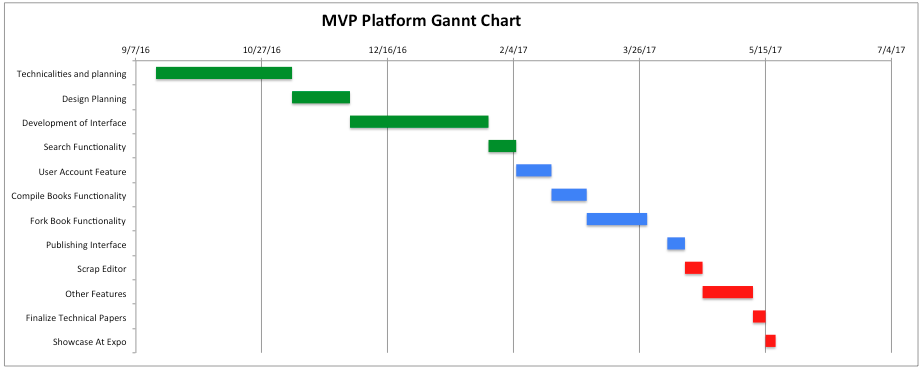
\includegraphics[width=160mm]{gantt_chart.png}
\caption{A preliminary Gantt Chart that outlines a rough sketch of our anticipated working time line as of Fall term}
\end{figure}

\subsection{Design Languages}
{\noindent This document will use UML as the design language.\par}





\clearpage
%Section 6
\section{Design Viewpoints}

\subsection{Introduction}
{\noindent This section will cover: context, composition, logical, dependency, information, interface, and interaction viewpoints. \par}

{\noindent Steven Powers is covering User Interface Tools, User Login \& Authentication, and Interface Design.  \par}
{\noindent Evan Tschuy is covering Server Back-end, Text Formatting, and Password Storage.  \par}
{\noindent Josh Matteson is covering Testing, Revision Control Software, and Database.  \par}


%Steven's Section

\subsection{Viewpoint: User Interface Tools}
{\noindent By: Steven Powers \par}

\subsubsection{Interface}
{\noindent The user interface is one of the most important parts to the Many
Voices Publishing Platform. An easy to use UI can make the difference between
two competing software solutions. The Many Voices Publishing Platform will be
interacted through a website that will display a users documents and their current
document. The User Interface Tools will allow for a high quality user experience
with a high number of screen repaints per second, further increasing the ease of use
with the software through a fluid user interface \cite{Eisenberg}.\par}

\subsubsection{Design Concerns}
{\noindent A poorly implemented UI can result in users choosing a competing
product or simply deciding not to use any software for their intended purpose.
Users are often impatient and quick to abandon software,
further proving the need for a robust and easy to use User Interface Toolset.  \par}

\subsubsection{Design Elements}
{\noindent The User Interface Tools will allow for scalability when it comes to
using the software on different platforms, including mobile, and desktop environments.
Additionally the tools will provide great interact-ability for the user.\par}

\subsubsection{Function Attribute}
{\noindent This component provides the user interface for users to interact with while using the software.
Handles display of information and provides the interface for input.  \par}

\subsubsection{Relationship}


\subsection{Viewpoint: User Login \& Authentication}
{\noindent By: Steven Powers  \par}

\subsubsection{Context--Dependency}
{\noindent A user login system is standard affair for most websites on the Internet.
How these user logins take place and authenticate users can vary quite
significantly depending on the implementation.
User login security is important for protecting the customer as well as
the reputation of the software and company. User Login \& Authentication
are dependent on Evan Tschuy's section on Password Storage section. \par}

\subsubsection{Design Concerns}
{\noindent Handling user logins and user authentication can be quite a painstaking process,
as any mistake can cost you customers and any reputation that was present
before the mistake was exploited. Authentication, or the matching of user submitted
data with our stored credentials can be exploited though a simple MySQL command,
if our servers are not secured properly. In house solutions can be buggy, or not as secure.
Third party solutions require an account with those services and has security in their hands. \par}

\subsubsection{Design Elements}
{\noindent A way to login securely, through created credentials or through a
third party login system, such as Login with Facebook or Google.  \par}

\subsubsection{Function Attribute}
{\noindent This component provides the functionality of user login process
and user authentication within the software.\par}

\subsubsection{Relationship}



\subsection{Viewpoint: Interface Design}
{\noindent By: Steven Powers \par}

\subsubsection{Information}
{\noindent The approach for user interface design is quite different
than that of the tools being used. Interface Design refers to the
methodologies employed to create the UI. This often takes the form of
user studies, and demoing of prototypes and release candidate mockups
for feedback. For our software, our target audience is professors,
especially those interested in publishing their own book currently or
in the near future. Using the target audience as a design requirement,
the designer is able to gleam a lot of information about how to best
serve this user.
Methodologies include user centered design, activity centered design,
and self design principles to list a few common disciplines.   \par}

\subsubsection{Design Concerns}
{\noindent Interface Design is an often overlooked portion of any software product.
For some software products it would be no surprise that the software is never
used in house, we are trying to avoid this feeling.
User centered design, while often the standard for the Computer Science industry, it
very costly, both in terms of time and money. There is a large amount of time into
user research studies and live demos. Self design, while much faster,
and easier to perform, can lead to results that do not satisfy your users expectations.\par}

\subsubsection{Design Elements}
{\noindent An Interface Design methodology that allows for efficient
use of time as well as successful design choices to best suit our users. \par}

\subsubsection{Function Attribute}
{\noindent Provides methodologies for improving Interface Design to assist
users and developers. \par}

\subsubsection{Relationship}






%Evan's Section
\newpage
\subsection{Viewpoint: Server Back-end}
{\noindent By: Evan Tschuy \par}

\subsubsection{ViewpointName}
{\noindent  \par}

\subsubsection{Design Concerns}
{\noindent  \par}

\subsubsection{Design Elements}
{\noindent  \par}

\subsubsection{Function Attribute}
{\noindent  \par}

\subsubsection{Relationship}


\subsection{Viewpoint: Text Formatting}
{\noindent By: Evan Tschuy \par}

\subsubsection{ViewpointName}
{\noindent  \par}

\subsubsection{Design Concerns}
{\noindent  \par}

\subsubsection{Design Elements}
{\noindent  \par}

\subsubsection{Function Attribute}
{\noindent  \par}

\subsubsection{Relationship}


\subsection{Viewpoint: Password Storage}
{\noindent By: Evan Tschuy \par}

\subsubsection{ViewpointName}
{\noindent  \par}

\subsubsection{Design Concerns}
{\noindent  \par}

\subsubsection{Design Elements}
{\noindent  \par}

\subsubsection{Function Attribute}
{\noindent  \par}

\subsubsection{Relationship}






%Josh's Section
\newpage
\subsection{Viewpoint: Testing}
{\noindent By: Josh Matteson \par}

\subsubsection{ViewpointName}
{\noindent  \par}

\subsubsection{Design Concerns}
{\noindent  \par}

\subsubsection{Design Elements}
{\noindent  \par}

\subsubsection{Function Attribute}
{\noindent  \par}

\subsubsection{Relationship}


\subsection{Viewpoint: Revision Control Software}
{\noindent By: Josh Matteson \par}

\subsubsection{ViewpointName}
{\noindent  \par}

\subsubsection{Design Concerns}
{\noindent  \par}

\subsubsection{Design Elements}
{\noindent  \par}

\subsubsection{Function Attribute}
{\noindent  \par}

\subsubsection{Relationship}


\subsection{Viewpoint: Database}
{\noindent By: Josh Matteson \par}

\subsubsection{ViewpointName}
{\noindent  \par}

\subsubsection{Design Concerns}
{\noindent  \par}

\subsubsection{Design Elements}
{\noindent  \par}

\subsubsection{Function Attribute}
{\noindent  \par}

\subsubsection{Relationship}







\newpage

%Section 7
\section{Annex A - (information Bibliography}

\nocite{*}
\bibliographystyle{IEEEtran}
\bibliography{designdocument}


%Section 8
%\section{Annex B - Conforming design language description}
%{\noindent \par}

%Section 9
%\section{Annex C - Templates for an SDD}
%{\noindent \par}


%Section 10
\newpage
\section{Conclusion}
{\noindent  The Many Voices Publishing Platform is a combination of User Interfaces, Documentation, User Centered Design, Testing, User Authentication, Databases, Server Back-end, Text Formatting, Password Storage, and the users themselves. Determining the technologies behind these parts and pieces is a difficult task to accomplish, as many choices can satisfy the requirements of the project. Finding the best solution however is the goal of this document, to provide a clear path forward for the platform as a whole. \par}


\newpage
\section{Signature Page}
\vspace{5pc}


\centering

\begin{tabular}{lllll}
Dr. Carlos Jensen, Client
& \_\_\_\_\_\_\_\_\_\_\_\_\_\_\_\_\_\_\_\_\_\_\_\_\_\_\_\_\_\_\_\_\_\_
& Date & \_\_\_\_\_\_\_\_\_\_\_\_\_\_\_\_\_\_\_\_\_ &  \\
& & & &  \\ \\
Steven Powers, Developer
& \_\_\_\_\_\_\_\_\_\_\_\_\_\_\_\_\_\_\_\_\_\_\_\_\_\_\_\_\_\_\_\_\_\_
& Date & \_\_\_\_\_\_\_\_\_\_\_\_\_\_\_\_\_\_\_\_\_ &  \\
& & & &  \\ \\
Josh Matteson, Developer
& \_\_\_\_\_\_\_\_\_\_\_\_\_\_\_\_\_\_\_\_\_\_\_\_\_\_\_\_\_\_\_\_\_\_
& Date & \_\_\_\_\_\_\_\_\_\_\_\_\_\_\_\_\_\_\_\_\_ &  \\
& & & &  \\ \\
Evan Tschuy, Developer
& \_\_\_\_\_\_\_\_\_\_\_\_\_\_\_\_\_\_\_\_\_\_\_\_\_\_\_\_\_\_\_\_\_\_
& Date & \_\_\_\_\_\_\_\_\_\_\_\_\_\_\_\_\_\_\_\_\_ &  \\
& & & &
\end{tabular}

\end{document}
